% !TEX program = xelatex
\PassOptionsToPackage{no-math}{fontspec}
\documentclass[a4paper,twocolumn,zihao=5,fontset=none,UTF8]{ctexart}
% Shared layout for the two Lab0 translations: Chinese two-column conference style.
\usepackage[a4paper,left=1.9cm,right=1.9cm,top=2.4cm,bottom=2.2cm,
  columnsep=0.7cm,headsep=0.5cm]{geometry}
\usepackage{amsmath,amssymb,bm}
\setmainfont{Times New Roman}
\setsansfont{Helvetica}
\setmonofont{Menlo}[Scale=0.85]
% macOS system CJK fonts; Kai/Fang come from TeX Live's Fandol set.
\setCJKmainfont{Songti SC}[BoldFont={Heiti SC},ItalicFont={FandolKai-Regular.otf}]
\setCJKsansfont{Heiti SC}
\setCJKmonofont{Heiti SC}
\setCJKfamilyfont{zhhei}{Heiti SC}
\setCJKfamilyfont{zhkai}{FandolKai-Regular.otf}
\setCJKfamilyfont{zhfs}{FandolFang-Regular.otf}
\providecommand{\heiti}{\CJKfamily{zhhei}}
\providecommand{\kaishu}{\CJKfamily{zhkai}}
\providecommand{\fangsong}{\CJKfamily{zhfs}}
\usepackage{newtxmath}
% fontspec's text fonts have no OT1 shapes; point math alphabets at newtx's Times.
\DeclareMathAlphabet{\mathrm}{OT1}{ntxtlf}{m}{n}
\DeclareMathAlphabet{\mathbf}{OT1}{ntxtlf}{b}{n}
\DeclareMathAlphabet{\mathtt}{OT1}{txtt}{m}{n}
\DeclareMathAlphabet{\mathsf}{OT1}{phv}{m}{n}
\SetSymbolFont{operators}{normal}{OT1}{ntxtlf}{m}{n}
\SetSymbolFont{operators}{bold}{OT1}{ntxtlf}{b}{n}
\usepackage{graphicx,booktabs,multirow,array}
\usepackage[font=small,labelsep=quad,skip=4pt]{caption}
\usepackage{enumitem}
\usepackage{fancyvrb}
\usepackage{fancyhdr}
\usepackage{xurl}
\usepackage[hidelinks]{hyperref}
\graphicspath{{figures/}}
\urlstyle{same}

\ctexset{
  section={format=\heiti\zihao{-4}\raggedright,beforeskip=1.2ex plus .3ex,
    afterskip=.8ex plus .2ex,aftername=\quad},
  subsection={format=\heiti\zihao{5}\raggedright,beforeskip=.9ex plus .2ex,
    afterskip=.5ex plus .1ex,aftername=\quad},
}
\setlist{nosep,leftmargin=2em}
\setlength{\parskip}{0pt}
\linespread{1.18}
\setlength{\abovedisplayskip}{5pt plus 2pt minus 2pt}
\setlength{\belowdisplayskip}{5pt plus 2pt minus 2pt}
\setlength{\textfloatsep}{10pt plus 2pt minus 3pt}
\setlength{\dbltextfloatsep}{10pt plus 2pt minus 3pt}
\emergencystretch=1em

% Bold run-in heading used by both papers ("Photogrammetric calibration." etc.).
\newcommand{\runin}[1]{\textbf{\heiti #1}\quad}
% Translator's note in a footnote.
\newcommand{\yizhe}[1]{\footnote{\kaishu 译者注：#1}}

\pagestyle{fancy}
\fancyhf{}
\renewcommand{\headrulewidth}{0.4pt}
\fancyfoot[C]{\small\thepage}


\fancyhead[L]{\small 机器人学集成小组项目 1 \quad Lab0-2 论文翻译}
\fancyhead[R]{\small Fusiello 等：一种紧凑的立体图像对校正算法}

\newcommand{\bP}{\widetilde{\mathbf{P}}}
\newcommand{\Q}{\mathbf{Q}}
\newcommand{\tq}{\widetilde{\mathbf{q}}}
\newcommand{\A}{\mathbf{A}}
\newcommand{\R}{\mathbf{R}}
\newcommand{\tv}{\mathbf{t}}
\newcommand{\w}{\mathbf{w}}
\newcommand{\cc}{\mathbf{c}}
\newcommand{\rr}{\mathbf{r}}
\newcommand{\tm}{\widetilde{\mathbf{m}}}
\newcommand{\tw}{\widetilde{\mathbf{w}}}
\newcommand{\pt}[1]{\mathsf{#1}}
\newcommand{\sci}[2]{#1{\cdot}10^{#2}}

\begin{document}

\twocolumn[{%
\begin{center}
  {\heiti\zihao{2} 一种紧凑的立体图像对校正算法\par}
  \vspace{0.5em}
  {\zihao{-4} A compact algorithm for rectification of stereo pairs\par}
  \vspace{0.8em}
  {\fangsong\zihao{4} Andrea Fusiello$^{1}$,\quad Emanuele Trucco$^{2}$,\quad Alessandro Verri$^{3}$\par}
  \vspace{0.4em}
  {\zihao{-5}\linespread{1.3}\selectfont
   1.\ 维罗纳大学科学与技术系，Ca' Vignal 2, Strada Le Grazie, 37134 Verona, Italy；e-mail: fusiello@sci.univr.it\\
   2.\ 赫瑞-瓦特大学计算与电气工程系，英国爱丁堡\qquad
   3.\ INFM，热那亚大学计算机与信息科学系，意大利热那亚\\
   收稿日期：1999 年 2 月 25 日\quad 录用日期：2000 年 3 月 2 日\quad 通信作者：A. Fusiello\par}
\end{center}
\vspace{0.4em}
{\zihao{-5}\linespread{1.25}\selectfont
\noindent{\heiti 摘\quad 要：}本文提出一种适用于一般的、无约束的立体装置的线性校正算法。该算法以两台原始相机的透视投影矩阵为输入，计算出一对校正后的投影矩阵。算法十分紧凑（仅 22 行 MATLAB 代码），且易于复现。我们报告的测试证明了该方法行为正确，并表明直接由校正后的图像进行三维重建时，精度的下降可以忽略不计。

\vspace{0.3em}
\noindent{\heiti 关键词：}校正；立体视觉；对极几何
\par}
\vspace{1.2em}
}]

{\renewcommand{\thefootnote}{}\footnotetext{\kaishu 原文：A.~Fusiello, E.~Trucco, A.~Verri. A compact algorithm for rectification of stereo pairs. \textit{Machine Vision and Applications}, 2000, 12: 16--22. \textcopyright\ Springer-Verlag 2000. 译者：许轩烨（学号 24020036071 / H00490299）。原文采用作者—年份制引用，译文按中文会议论文惯例改为顺序编号制，编号按参考文献表的字母顺序排列；公式与图号与原文一致。}}

\section{引言与研究动机}

给定一对立体图像，\emph{校正}（rectification）就是为每个像平面确定一个变换，使得共轭极线对变为共线，并且平行于某一条图像坐标轴（通常是水平轴）。校正后的图像可以看作由一个新的立体装置采集得到，而这个新装置是通过旋转原始相机得到的。校正的重要优点在于，它使立体对应点的计算[3]更为简单，因为搜索只需沿校正后图像的水平线进行。

我们假设立体装置已经标定，即相机的内部参数以及两者的相对位置和朝向均已知。这一假设并非绝对必要，但能使技术更为简单。另一方面，在由稠密立体视觉重建物体的三维形状时，标定在实践中是必需的，而且在许多情形下都可以用多种算法完成[2, 13]。

校正是立体视觉中的经典问题；然而据我们所知，计算机视觉文献中可用的方法并不多。Ayache 和 Lustman[1]提出了一种校正算法，其中需要手工构造一个满足若干约束的矩阵，而哪些约束是必要的、哪些是任意的，其区分并不清楚。一些作者在限制性的假设下讨论校正问题，例如 Papadimitriou 和 Dennis[11]假设了一种限制性很强的几何结构（两相机参考坐标系的竖直轴相互平行）。近来，Hartley 和 Gupta[7]、Robert 等[14]以及 Hartley[6]提出了针对\emph{弱标定}立体装置的校正算法，所谓弱标定，是指只给出图像之间点对应关系的装置。

本文手稿完成之后发表的最新工作包括 Loop 和 Zhang[10]、Isgr\`o 和 Trucco[9]以及 Pollefeys 等[12]。其中一些工作还关注如何使校正图像的畸变最小。我们不讨论这一问题，部分原因是在已标定情形下，这种畸变不如弱标定情形严重。

本文提出一种新算法，用于校正安装一般相机、几何结构无约束的已标定立体装置。我们的工作改进并扩展了 Ayache 和 Lustman[1]的工作：得到的结果基本相同，但方式更紧凑、更清晰。算法简单，并给出了全部细节。此外，鉴于易于复现、易于获取且表述清晰的算法较为缺乏，我们已将代码公开在网上。

\section{相机模型与对极几何}

本节简要回顾本文所需的透视投影数学背景，更多细节参见 Faugeras[4]。

\subsection{相机模型}

针孔相机由其\emph{光心} $\pt{C}$ 和\emph{视网膜平面}（或\emph{像平面}）$\mathcal{R}$ 建模。三维点 $\pt{W}$ 投影为图像点 $\pt{M}$，$\pt{M}$ 是 $\mathcal{R}$ 与经过 $\pt{C}$ 和 $\pt{W}$ 的直线的交点。经过 $\pt{C}$ 且垂直于 $\mathcal{R}$ 的直线称为\emph{光轴}，光轴与 $\mathcal{R}$ 的交点称为\emph{主点}。$\pt{C}$ 到 $\mathcal{R}$ 的距离称为\emph{焦距}。

设 $\w=[x\ y\ z]^\top$ 为 $\pt{W}$ 在（任意固定的）世界参考坐标系中的坐标，$\mathbf{m}=[u\ v]^\top$ 为 $\pt{M}$ 在像平面中的坐标（以像素计）。从三维坐标到二维坐标的映射是\emph{透视投影}，它可以用\emph{齐次坐标}下的线性变换表示。设 $\tm=[u\ v\ 1]^\top$ 和 $\tw=[x\ y\ z\ 1]^\top$ 分别为 $\pt{M}$ 和 $\pt{W}$ 的齐次坐标，则透视变换由矩阵 $\bP$ 给出：
\begin{equation}
  \tm\cong\bP\tw,
\end{equation}
其中 $\cong$ 表示在相差一个尺度因子的意义下相等。因此，相机由其\emph{透视投影矩阵}（perspective projection matrix，下文简称 PPM）$\bP$ 建模。利用 QR 分解，$\bP$ 可以分解为如下乘积：
\begin{equation}
  \bP=\A[\R\mid\tv].
\end{equation}
矩阵 $\A$ 只取决于\emph{内部参数}，其形式为
\begin{equation}
  \A=\begin{bmatrix}\alpha_u & \gamma & u_0\\ 0 & \alpha_v & v_0\\ 0 & 0 & 1\end{bmatrix},
\end{equation}
其中 $\alpha_u=-fk_u$、$\alpha_v=-fk_v$ 分别为以水平像素和竖直像素为单位的焦距（$f$ 为以毫米为单位的焦距，$k_u$ 和 $k_v$ 分别为沿 $u$ 轴和 $v$ 轴每毫米的有效像素数），$(u_0,v_0)$ 为\emph{主点}坐标，即光轴与视网膜平面的交点，$\gamma$ 为\emph{倾斜}因子，用于描述 $u$、$v$ 轴不正交的情况。

相机的位置和朝向（\emph{外部参数}）由 $3\times3$ 旋转矩阵 $\R$ 和平移向量 $\tv$ 编码，它们表示将相机参考坐标系变换到世界参考坐标系的刚体变换。

将 PPM 写为
\begin{equation}
  \bP=\left[\begin{array}{c|c}\mathbf{q}_1^\top & q_{14}\\ \mathbf{q}_2^\top & q_{24}\\ \mathbf{q}_3^\top & q_{34}\end{array}\right]=[\Q\mid\tq].
\end{equation}
在笛卡儿坐标下，投影（式 (1)）可写为
\begin{equation}
  \left\{\begin{aligned}
    u&=\frac{\mathbf{q}_1^\top\w+q_{14}}{\mathbf{q}_3^\top\w+q_{34}}\\[2pt]
    v&=\frac{\mathbf{q}_2^\top\w+q_{24}}{\mathbf{q}_3^\top\w+q_{34}}.
  \end{aligned}\right.
\end{equation}

\emph{焦平面}是与视网膜平面平行且包含光心 $\pt{C}$ 的平面。$\pt{C}$ 的坐标 $\cc$ 为
\begin{equation}
  \cc=-\Q^{-1}\tq.
\end{equation}
因此，$\bP$ 可以写为
\begin{equation}
  \bP=[\Q\mid-\Q\cc].
\end{equation}

与图像点 $\pt{M}$ 相关联的\emph{光线}是直线 $\pt{M}\pt{C}$，即三维点集 $\{\w:\tm\cong\bP\tw\}$。其参数形式为
\begin{equation}
  \w=\cc+\lambda\Q^{-1}\tm,\qquad \lambda\in\mathbb{R}.
\end{equation}

\begin{figure}[t]
  \centering
  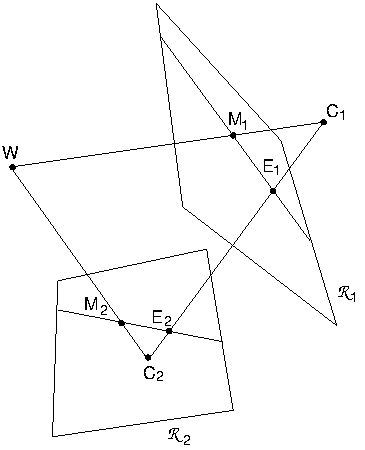
\includegraphics[width=0.66\linewidth]{fusiello_fig1}
  \caption{对极几何。第一台相机的极点 $\pt{E}_1$ 是第二台相机光心 $\pt{C}_2$ 的投影（反之亦然）}
\end{figure}

\subsection{对极几何}

考虑由两台针孔相机组成的立体装置（图 1）。设 $\pt{C}_1$ 和 $\pt{C}_2$ 分别为左、右相机的光心。三维点 $\pt{W}$ 投影到两个像平面上，得到点 $\pt{M}_1$ 和 $\pt{M}_2$，它们构成一对\emph{共轭点}。给定左像平面中的点 $\pt{M}_1$，其在右图像中的共轭点被约束在一条直线上，这条直线称为（$\pt{M}_1$ 的）\emph{极线}。由于 $\pt{M}_1$ 可以是其光线上任意一点的投影，极线就是 $\pt{M}_1$ 的光线经 $\pt{C}_2$ 所成的投影。一个像平面中的所有极线都经过一个公共点（分别为 $\pt{E}_1$ 和 $\pt{E}_2$），该点称为\emph{极点}，它是另一台相机光心的投影。

当 $\pt{C}_1$ 位于右相机的焦平面内时，右极点位于无穷远处，右图像中的极线构成一族平行线。一种非常特殊的情况是两个极点都位于无穷远处，这发生在直线 $\pt{C}_1\pt{C}_2$（即\emph{基线}）同时包含于两个焦平面内时，即两个视网膜平面都平行于基线。此时，两幅图像中的极线都构成一族平行线。任何一对图像都可以经过变换，使每幅图像中的极线都平行且水平，这一过程称为\emph{校正}。

\section{相机矩阵的校正}

我们假设立体装置\emph{已标定}，即 PPM $\bP_{o1}$ 和 $\bP_{o2}$ 已知。校正的思想是定义两个新的 PPM $\bP_{n1}$ 和 $\bP_{n2}$：它们由旧 PPM 绕各自光心旋转得到，直到两个焦平面共面，从而都包含基线。这保证了极点位于无穷远处，因此极线是\emph{平行}的。为了得到\emph{水平}的极线，基线必须平行于两台相机新的 $\pt{X}$ 轴。此外，为了实现正确的校正，共轭点必须具有\emph{相同的竖直坐标}，这可以通过要求新相机具有相同的内部参数来实现。注意，由于焦距相同，两个视网膜平面也共面，如图 2 所示。

\begin{figure}[t]
  \centering
  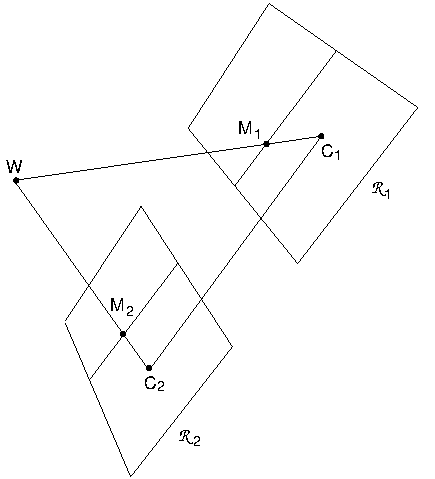
\includegraphics[width=0.66\linewidth]{fusiello_fig2}
  \caption{校正后的相机。两个视网膜平面共面且平行于基线}
\end{figure}

总之：新 PPM 的位置（即光心）与旧相机相同，而新的朝向（两台相机相同）与旧朝向相差适当的旋转；两台相机的内部参数相同。因此，得到的两个 PPM 仅在光心上有所不同，可以把它们看作同一台相机沿其参考坐标系的 $\pt{X}$ 轴平移的结果。

我们用分解形式写出新 PPM。由式 (2) 和式 (7) 得
\begin{equation}
  \bP_{n1}=\A[\R\mid-\R\,\cc_1],\qquad \bP_{n2}=\A[\R\mid-\R\,\cc_2].
\end{equation}
内部参数矩阵 $\A$ 对两个 PPM 相同，可以任意选取（见 MATLAB 代码）。光心 $\cc_1$ 和 $\cc_2$ 取旧的光心，由式 (6) 计算。给出相机姿态的矩阵 $\R$ 对两个 PPM 也相同，我们用其行向量来确定它：
\begin{equation}
  \R=\begin{bmatrix}\rr_1^\top\\ \rr_2^\top\\ \rr_3^\top\end{bmatrix},
\end{equation}
这些行向量分别是相机参考坐标系的 $\pt{X}$、$\pt{Y}$、$\pt{Z}$ 轴在世界坐标系中的表示。

根据前面的讨论，我们取：
\begin{enumerate}
  \item 新 $\pt{X}$ 轴平行于基线：$\rr_1=(\cc_1-\cc_2)/\|\cc_1-\cc_2\|$；
  \item 新 $\pt{Y}$ 轴垂直于 $\pt{X}$（必须满足）且垂直于 $\mathbf{k}$：$\rr_2=\mathbf{k}\wedge\rr_1$；
  \item 新 $\pt{Z}$ 轴垂直于 $\pt{XY}$ 平面（必须满足）：$\rr_3=\rr_1\wedge\rr_2$。
\end{enumerate}
第 2 点中，$\mathbf{k}$ 是一个任意单位向量，它确定新 $\pt{Y}$ 轴在垂直于 $\pt{X}$ 的平面内的位置。我们取 $\mathbf{k}$ 等于旧左相机矩阵的 $\pt{Z}$ 轴单位向量，从而约束新 $\pt{Y}$ 轴同时垂直于新 $\pt{X}$ 轴和旧左相机的 $\pt{Z}$ 轴。

当光轴平行于基线，即存在纯前向运动时，该算法失效。

在文献[5]中，我们对校正的要求进行了解析的形式化描述，并证明了本节给出的算法满足这些要求。

\section{校正变换}

为了校正（比如说）左图像，我们需要计算把 $\bP_{o1}=[\Q_{o1}\mid\tq_{o1}]$ 的像平面映射到 $\bP_{n1}=[\Q_{n1}\mid\tq_{n1}]$ 的像平面的变换。我们将看到，所求的变换是由 $3\times3$ 矩阵 $\mathbf{T}_1=\Q_{n1}\Q_{o1}^{-1}$ 给出的共线变换。同样的结论也适用于右图像。

对任意三维点 $\w$，可以写出
\begin{equation}
  \left\{\begin{aligned}
    \tm_{o1}&\cong\bP_{o1}\tw\\
    \tm_{n1}&\cong\bP_{n1}\tw.
  \end{aligned}\right.
\end{equation}
根据式 (8)，由于校正不移动光心，光线方程为
\begin{equation}
  \left\{\begin{aligned}
    \w&=\cc_1+\lambda_o\Q_{o1}^{-1}\tm_{o1}, & \lambda_o&\in\mathbb{R}\\
    \w&=\cc_1+\lambda_n\Q_{n1}^{-1}\tm_{n1}, & \lambda_n&\in\mathbb{R};
  \end{aligned}\right.
\end{equation}
因此
\begin{equation}
  \tm_{n1}=\lambda\Q_{n1}\Q_{o1}^{-1}\tm_{o1},\qquad \lambda\in\mathbb{R}.
\end{equation}

然后将变换 $\mathbf{T}_1$ 作用于原始左图像，得到校正后的图像，如图 5 所示。注意，校正图像中的像素（整数坐标位置）一般对应于原始像平面上的非整数位置。因此，校正图像的灰度值通过双线性插值计算。

三维点可以直接由校正后的图像，利用 \texttt{Pn1}、\texttt{Pn2} 通过三角测量[8]重建。

\section{校正算法小结}

鉴于立体视觉在研究和应用中的广泛普及，我们力求使算法尽可能易于复现和使用。为此，我们给出算法的可运行 MATLAB 代码。代码简单紧凑（22 行），所附注释使不了解 MATLAB 的读者也能读懂\footnote{译文将代码注释译为中文，代码本身与原文一致。}。\texttt{rectify} 函数（见 MATLAB 代码）的用法如下：
\begin{itemize}[label=--]
  \item 给定一对立体图像 \texttt{I1}、\texttt{I2} 以及（由标定得到的）PPM \texttt{Po1}、\texttt{Po2}；
  \item 计算 \texttt{[T1,T2,Pn1,Pn2]=rectify(Po1,Po2)}；
  \item 分别施加 \texttt{T1} 和 \texttt{T2} 校正两幅图像。
\end{itemize}

\begin{Verbatim}[fontsize=\small,xleftmargin=0.3em,frame=lines,framesep=4pt]
function [T1,T2,Pn1,Pn2] = rectify(Po1,Po2)

% RECTIFY：计算校正矩阵

% 分解旧的 PPM
[A1,R1,t1] = art(Po1);
[A2,R2,t2] = art(Po2);

% 光心（保持不变）
c1 = - inv(Po1(:,1:3))*Po1(:,4);
c2 = - inv(Po2(:,1:3))*Po2(:,4);

% 新 x 轴（= 基线方向）
v1 = (c1-c2);
% 新 y 轴（垂直于新 x 轴和旧 z 轴）
v2 = cross(R1(3,:)',v1);
% 新 z 轴（垂直于基线和 y 轴）
v3 = cross(v1,v2);

% 新的外部参数
R = [v1'/norm(v1)
     v2'/norm(v2)
     v3'/norm(v3)];
% 平移保持不变

% 新的内部参数（任意选取）
A = (A1 + A2)./2;
A(1,2)=0; % 无倾斜

% 新的投影矩阵
Pn1 = A * [R -R*c1 ];
Pn2 = A * [R -R*c2 ];

% 校正图像变换
T1 = Pn1(1:3,1:3)* inv(Po1(1:3,1:3));
T2 = Pn2(1:3,1:3)* inv(Po2(1:3,1:3));

% ------------------------

function [A,R,t] = art(P)
% ART：将 PPM 分解为 P=A*[R;t]

Q = inv(P(1:3, 1:3));
[U,B] = qr(Q);

R = inv(U);
t = B*P(1:3,4);
A = inv(B);
A = A ./A(3,3);
\end{Verbatim}

包含该算法 C 和 MATLAB 实现、数据集和文档的“校正工具包”可在网上获取\footnote{\url{http://www.sci.univr.it/~fusiello/rect.html}}。

\section{实验结果}

我们进行了测试，以验证算法能正确地完成校正，同时检验直接由校正后的图像进行三维重建时精度不会下降。

\begin{figure}[t]
  \centering
  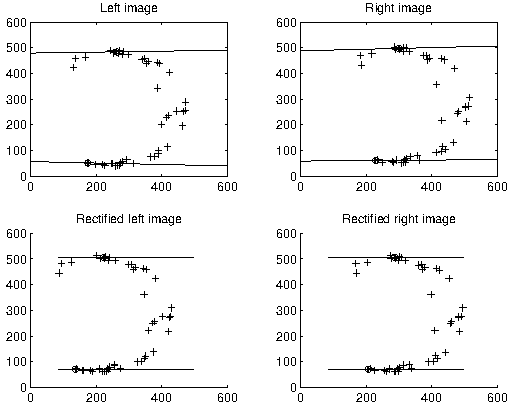
\includegraphics[width=\linewidth]{fusiello_fig3}
  \caption{近似已校正的合成立体图像对（\emph{上}）及校正后的图像对（\emph{下}）。图中画出了两幅图像中以\emph{圆圈}标记的点所对应的极线}
  \vspace{6pt}
  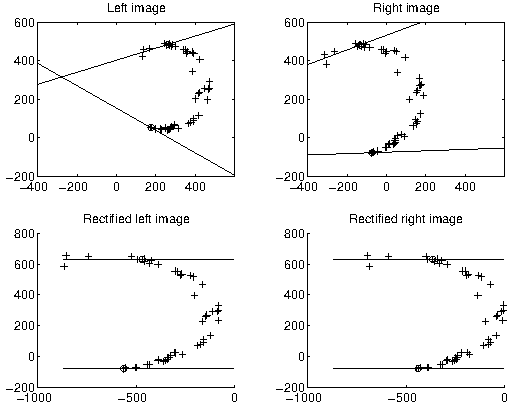
\includegraphics[width=\linewidth]{fusiello_fig4}
  \caption{一般的合成立体图像对（\emph{上}）及校正后的图像对（\emph{下}）。图中画出了两幅图像中以\emph{圆圈}标记的点所对应的极线}
\end{figure}

\runin{正确性。}测试同时使用了合成数据和真实数据。每组合成数据由一个三维点云和一对 PPM 组成。限于篇幅，我们只报告两个例子。图 3 给出了近似已校正立体装置的原始图像和校正后图像：相机平移为 $-[100\ 2\ 3]$\,mm，旋转角为横滚角（roll）$1.5^\circ$、俯仰角（pitch）$2^\circ$、偏航角（yaw）$1^\circ$。图 4 给出了更一般几何结构下的相同结果：相机平移为 $-[100\ 20\ 30]$\,mm，旋转角为横滚角 $19^\circ$、俯仰角 $32^\circ$、偏航角 $5^\circ$。

真实数据实验使用了 INRIA-Syntim 提供的已标定立体图像对。我们给出了近似已校正的立体装置（图 5）和更一般的立体几何结构（图 6）下得到的结果。校正后图像的像素坐标并不受限于像平面的某个特定区域，因此我们对两幅图像施加了一个任意平移，把它们移到平面上合适的区域，然后将输出图像裁剪为输入图像的尺寸。对于“Sport”立体图像对（图像尺寸 $768\times576$），我们从以下相机矩阵出发：
{\small\setlength{\arraycolsep}{3pt}
\begin{equation*}
  \mathbf{P}_{o1}\!=\!\begin{bmatrix}
    \sci{9.765}{2} & \sci{5.382}{1} & -\sci{2.398}{2} & \sci{3.875}{5}\\
    \sci{9.849}{1} & \sci{9.333}{2} & \sci{1.574}{2} & \sci{2.428}{5}\\
    \sci{5.790}{-1} & \sci{1.108}{-1} & \sci{8.077}{-1} & \sci{1.118}{3}
  \end{bmatrix}\!,
\end{equation*}
\begin{equation*}
  \mathbf{P}_{o2}\!=\!\begin{bmatrix}
    \sci{9.767}{2} & \sci{5.376}{1} & -\sci{2.400}{2} & \sci{4.003}{4}\\
    \sci{9.868}{1} & \sci{9.310}{2} & \sci{1.567}{2} & \sci{2.517}{5}\\
    \sci{5.766}{-1} & \sci{1.141}{-1} & \sci{8.089}{-1} & \sci{1.174}{3}
  \end{bmatrix}\!.
\end{equation*}}
在 \texttt{rectify} 程序中加入语句 \texttt{A(1,3) = A(1,3) + 160}，使校正后的图像保持在 $768\times576$ 窗口的中央，得到如下校正后的相机矩阵：
{\small\setlength{\arraycolsep}{3pt}
\begin{equation*}
  \mathbf{P}_{n1}\!=\!\begin{bmatrix}
    \sci{1.043}{3} & \sci{7.452}{1} & -\sci{2.585}{2} & \sci{4.124}{5}\\
    \sci{1.165}{2} & \sci{9.338}{2} & \sci{1.410}{2} & \sci{2.388}{5}\\
    \sci{6.855}{-1} & \sci{1.139}{-1} & \sci{7.190}{-1} & \sci{1.102}{3}
  \end{bmatrix}\!,
\end{equation*}
\begin{equation*}
  \mathbf{P}_{n2}\!=\!\begin{bmatrix}
    \sci{1.043}{3} & \sci{7.452}{1} & -\sci{2.585}{2} & \sci{4.069}{4}\\
    \sci{1.165}{2} & \sci{9.338}{2} & \sci{1.410}{2} & \sci{2.388}{5}\\
    \sci{6.855}{-1} & \sci{1.139}{-1} & \sci{7.190}{-1} & \sci{1.102}{3}
  \end{bmatrix}\!.
\end{equation*}}

\begin{figure*}[t]
  \centering
  \begin{minipage}[t]{0.485\textwidth}
    \centering
    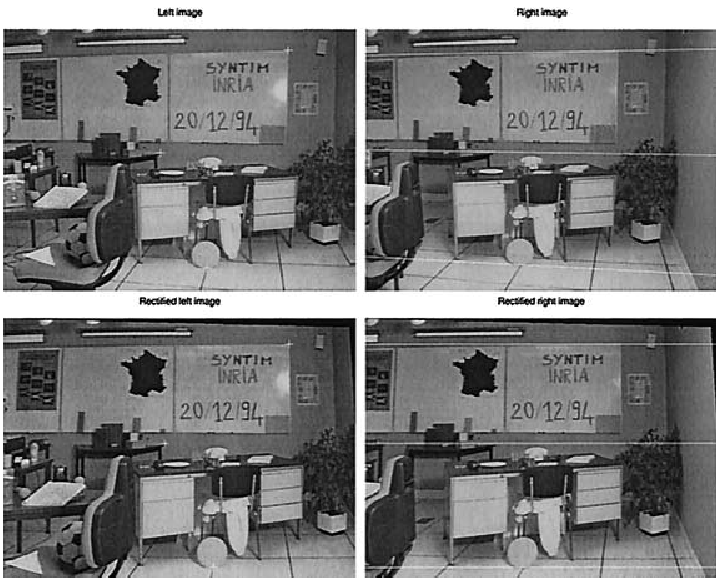
\includegraphics[width=\linewidth]{fusiello_fig5}
    \caption{“Sport”立体图像对（\emph{上}）及校正后的图像对（\emph{下}）。右侧图像中画出了与左侧图像中标记点相对应的极线}
  \end{minipage}\hfill
  \begin{minipage}[t]{0.485\textwidth}
    \centering
    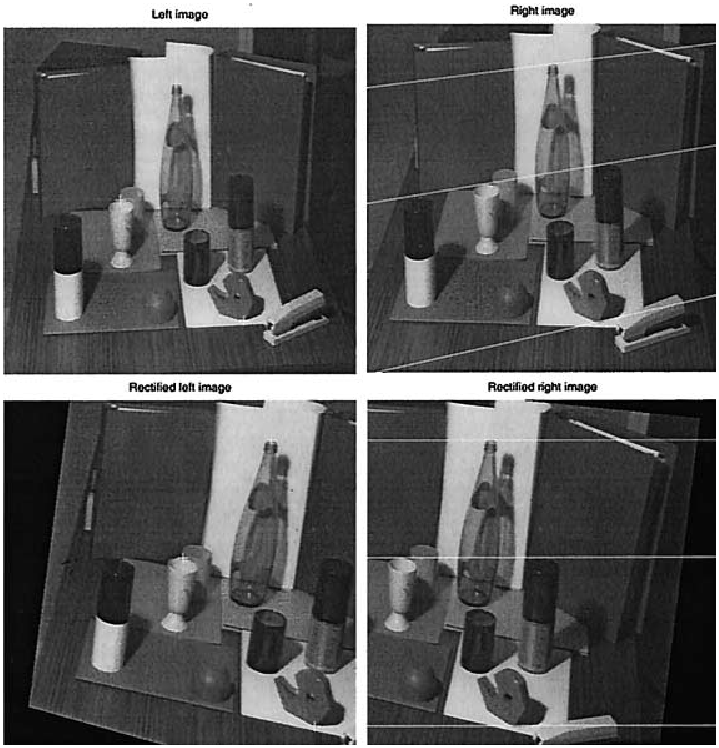
\includegraphics[width=0.78\linewidth]{fusiello_fig6}
    \caption{“Color”立体图像对（\emph{上}）及校正后的图像对（\emph{下}）。右侧图像中画出了与左侧图像中标记点相对应的极线}
  \end{minipage}
\end{figure*}

\begin{figure*}[t]
  \centering
  \begin{minipage}[t]{0.43\textwidth}
    \centering
    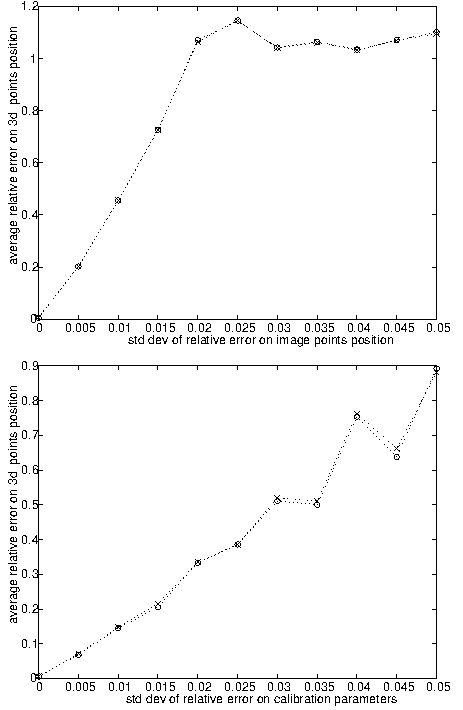
\includegraphics[width=0.9\linewidth]{fusiello_fig7}
    \caption{一般合成立体图像对的重建误差随图像坐标噪声水平（\emph{上}）和标定参数噪声水平（\emph{下}）的变化。\emph{叉号}表示由校正后图像重建的结果，\emph{圆圈}表示由未校正图像重建的结果}
  \end{minipage}\hspace{0.06\textwidth}
  \begin{minipage}[t]{0.43\textwidth}
    \centering
    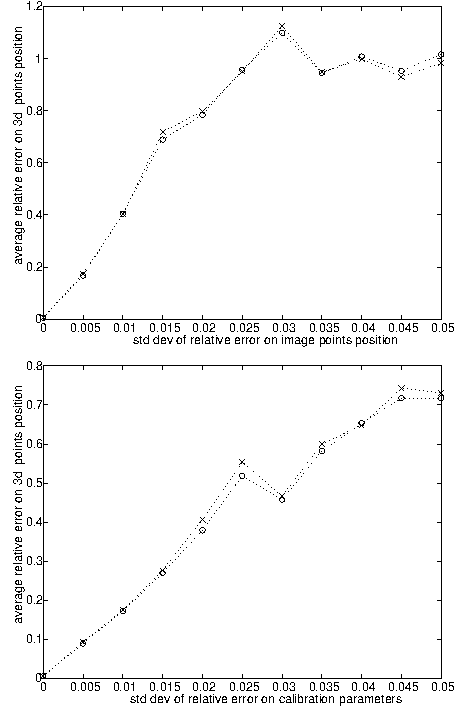
\includegraphics[width=0.9\linewidth]{fusiello_fig8}
    \caption{近似已校正合成立体图像对的重建误差随图像坐标噪声水平（\emph{上}）和标定参数噪声水平（\emph{下}）的变化。\emph{叉号}表示由校正后图像重建的结果，\emph{圆圈}表示由未校正图像重建的结果}
  \end{minipage}

  \vspace{2pt}
  \raggedright{\kaishu\small 译者注：原文图 7、图 8 的图注写作“（左）”“（右）”，但原文中两个子图实际为上下排列，译文按实际排版改为“（上）”“（下）”。}
\end{figure*}

\runin{精度。}为了评估校正对重建引入的误差，我们比较了由原始图像和由校正后图像计算得到的三维重建精度。我们使用了随机三维点云的含噪声合成图像。成像误差通过扰动图像坐标来模拟，标定误差通过扰动内部参数和外部参数来模拟，两者均采用加性高斯噪声。重建采用线性特征向量法（linear-eigen method）[8]。

图 7 和图 8 给出了三维点位置上测得的（在点集上平均的）相对误差随噪声变化的曲线。图 7 为图 4 所用立体装置的结果，图 8 为图 3 所用立体装置的结果。图中每个点都是 100 次独立试验的平均值。横坐标为图像点坐标或标定参数相对误差的标准差。

\section{结论}

如果图像经过校正，稠密立体匹配将大为简化。我们提出了一种简单的、易于理解和使用的算法，并通过解析推导和实验证明了其正确性。测试表明，与由原始图像重建相比，由校正后的图像重建不会引入可察觉的误差。我们相信，一个通用的校正算法，连同我们在网上公开的材料，能够成为研究界和应用界共同的有用资源。

\vspace{0.5em}
\noindent{\heiti 致谢}\quad 感谢 Bruno Caprile 的宝贵讨论，以及匿名审稿人提出的有益意见。本工作部分得到 British Council-MURST/CRUI 和 EPSRC（GR/L18716）的资助。立体图像对由 INRIA-Syntim 提供（版权所有）。

\section*{参考文献}
\begingroup
\small
\begin{enumerate}[label={[\arabic*]},leftmargin=2.2em,itemsep=1pt]
\item Ayache N, Lustman F (1991) Trinocular stereo vision for robotics. IEEE Trans Pattern Anal Mach Intell 13: 73--85
\item Caprile B, Torre V (1990) Using vanishing points for camera calibration. Int J Comput Vision 4: 127--140
\item Dhond UR, Aggarwal JK (1989) Structure from stereo -- a review. IEEE Trans Syst Man Cybern 19(6): 1489--1510
\item Faugeras O (1993) Three-Dimensional Computer Vision: A Geometric Viewpoint. The MIT Press, Cambridge, Mass.
\item Fusiello A, Trucco E, Verri A (1998) Rectification with unconstrained stereo geometry. Research Memorandum RM/98/12, CEE Dept., Heriot-Watt University, Edinburgh, UK. \url{ftp://ftp.sci.univr.it/pub/Papers/Fusiello/RM-98-12.ps.gz}
\item Hartley R (1999) Theory and practice of projective rectification. Int J Comput Vision 35(2): 1--16
\item Hartley R, Gupta R (1993) Computing matched-epipolar projections. In: CVPR93, New York, NJ, pp 549--555
\item Hartley RI, Sturm P (1997) Triangulation. Comput Vision Image Understanding 68(2): 146--157
\item Isgr\`o F, Trucco E (1999) Projective rectification without epipolar geometry. In: CVPR99, Fort Collins, CO, pp I:94--99
\item Loop C, Zhang Z (1999) Computing rectifying homographies for stereo vision. In: CVPR99, Fort Collins, CO, pp I:125--131
\item Papadimitriou DV, Dennis TJ (1996) Epipolar line estimation and rectification for stereo images pairs. IEEE Trans Image Process 3(4): 672--676
\item Pollefeys M, Koch R, VanGool L (1999) A simple and efficient rectification method for general motion. In: ICCV99, Corfu, Greece, pp 496--501
\item Robert L (1996) Camera calibration without feature extraction. Comput Vision, Graphics Image Process 63(2): 314--325
\item Robert L, Zeller C, Faugeras O, H\'ebert M (1997) Applications of non-metric vision to some visually guided robotics tasks. In: Aloimonos Y (ed) Visual Navigation: From Biological Systems to Unmanned Ground Vehicles, Chap.\,5. Lawrence Erlbaum Assoc., pp 89--134
\end{enumerate}
\endgroup

\section*{作者简介}
{\small
\noindent{\heiti Andrea Fusiello}\quad 1994 年获乌迪内大学（Universit\`a di Udine）计算机科学 Laurea（硕士）学位，1999 年获的里雅斯特大学（Universit\`a di Trieste）信息工程博士学位。1993—1994 年在 IRST（意大利特伦托）计算机视觉组工作，1996—1998 年在乌迪内大学机器视觉实验室工作。1998 年和 1999 年任英国赫瑞-瓦特大学计算与电气工程系访问研究员。现为维罗纳大学 DiST 研究助理（Research Associate）。他发表过实时任务调度、自主车辆导航、立体视觉和特征跟踪等方面的论文，目前的研究集中于三维计算机视觉及其在水下机器人中的应用。他是 IAPR 会员。

\noindent{\heiti Emanuele Trucco}\quad 1984 年以优异成绩（cum laude）获热那亚大学电子工程 Laurea（硕士）学位，1990 年获该校电子工程研究博士（PhD）学位。自 1984 年起，他先后在欧洲共同体委员会 EURATOM 联合研究中心（意大利伊斯普拉）以及热那亚大学和爱丁堡大学从事机器视觉研究，现任赫瑞-瓦特大学计算与电气工程系高级讲师。目前的研究兴趣为三维机器视觉及其应用，特别是在水下机器人中的应用。Trucco 博士已发表 80 余篇经同行评审的论文和一部三维视觉著作。他是 IEEE、英国机器视觉协会（BMVA）和 AISB 会员，也是 BMVA（苏格兰分会）和 IEE PG E4 的委员会成员。

\noindent{\heiti Alessandro Verri}\quad 1984 年和 1988 年分别获热那亚大学理论物理 Laurea 学位和博士学位。自 1989 年起任热那亚大学研究员（Ricercatore），先在物理系，自 1997 年秋起在计算机与信息科学系。他发表了约 50 篇关于人和机器视觉计算各方面问题的论文，内容包括立体视觉、运动分析、形状表示和物体识别，并合著了一部计算机视觉教材。他曾在 MIT、国际计算机科学研究所、INRIA/IRISA（雷恩）和赫瑞-瓦特大学任访问学者。目前的兴趣涵盖从模式识别与计算机视觉中计算问题的研究，到用于工业检测和质量控制的视觉系统的开发。
\par}

\end{document}
